\documentclass[10pt,a4paper]{article}
\setlength{\parskip}{0.8em}

\usepackage[utf8]{inputenc} % para poder usar tildes en archivos UTF-8
\usepackage[spanish]{babel} % para que comandos como \today den el resultado en castellano
\usepackage[left=2cm, right=2cm, top=2cm, bottom=2cm]{geometry}
\usepackage{caratula}

\usepackage{amsmath,amsfonts,amssymb,mathtools,amsthm,epsfig,epstopdf,url,array}
\usepackage{xcolor}
\usepackage{xspace}
\usepackage{xargs}
\usepackage{ifthen}
\usepackage{amsmath}
 
\usepackage{enumerate}
\usepackage{multirow}
\usepackage{float}

\usepackage{verbatim}


\usepackage{caption}

% \usepackage[onelanguage, spanish]{algorithm2e}
  % \NoCaptionOfAlgo
% \LinesNumbered\RestyleAlgo{ruled}\IncMargin{1em}\DontPrintSemicolon\SetArgSty{}\SetCommentSty{textsf}\SetFuncSty{textsf}
% \SetKwProg{For}{para}{ hacer}{fin}
% \SetKwProg{Fn}{función}{:}{fin}

\def\code#1{\texttt{#1}}

\usepackage{mathtools} 
\usepackage{changepage}
\usepackage{pdfpages}
\usepackage{hyperref}
\usepackage[page, toc]{appendix}
\usepackage[nottoc]{tocbibind}
\usepackage{subfigure}
\usepackage{graphicx}
\usepackage{euler}
\usepackage{listings}
\usepackage{tikz}
\usetikzlibrary{graphs,graphs.standard}
\usetikzlibrary{arrows}
\usepackage{algorithmicx, algpseudocode, algorithm}
\usepackage{float}

\newcommand{\norm}[1]{\left\lVert#1\right\rVert}
\newtheorem{theorem}{Theorem}[section]
\newtheorem{corollary}{Corollary}[theorem]
\newtheorem{lemma}[theorem]{Lemma}

\DeclareMathOperator{\tc}{\textbf{tc}}

\begin{document}

\titulo{Trabajo Práctico 2: Llenalo con super}

\materia{Algoritmos y estructuras de datos III}

\integrante{Martino, Maximiliano}{123/17}{maxii.martino@gmail.com}
\integrante{Blufstein, Marcos}{300/17}{mjblufstein@dc.uba.ar}
\integrante{Peretti, Olivia}{359/17}{operetti@dc.uba.ar}
\integrante{Pironio, Nicolás}{37/17}{npironio@dc.uba.ar}
\maketitle

\clearpage
\tableofcontents

\clearpage

\section{Introducci\'on}

En este trabajo resolveremos el problema de encontrar un camino para ir de una a ciudad a otra minimizando el costo del combustible. Para modelar el problema computacionalmente, utilizamos la siguiente representación: tendremos un grafo G, con n nodos y m aristas. Cada nodo representa una ciudad distinta y cada arista una ruta entre dos ciudades. Además cada arista $m_{j}$ tendrá asignado un valor $l_{j}$ que representa la cantidad de litros de nafta que necesita nuestro vehículo para recorrer dicha ruta. Por otro lado, cada nodo $n_{i}$  también tendrá un valor asignado $c_{i}$, que representa el costo de la nafta por litro en dicha ciudad. \\
\indent La capacidad del tanque de nuestro auto será de 60 litros, y nuestro algoritmo devolverá el costo mínimo de combustible partiendo de una ciudad y terminando en otra.\\
\indent Para resolver este problema implementaremos cuatro algoritmos distintos.
\begin{enumerate}
\item Algoritmo de Dijkstra.
\item Algoritmo de Dijkstra con cola de prioridad.
\item Algoritmo de Bellman-Ford.
\item Algoritmo de Floyd-Warshall.
\end{enumerate}

\indent El programa toma como entrada un archivo cuya primera línea debe tener dos enteros $n$ y $m$s correspondientes a la cantidad de ciudades y a la cantidad de rutas respectivamete. Luego habrá n líneas. Cada una con un entero $c_{i}$ que representa el costo del litro de combustible en la ciudad $i$. Luego deberán haber m líneas con tres entero $a_{i}$, $b_{i}$ y $l_{i}$. $a_{i}$ y $b_{i}$ indicarán las ciudades conectadas por la ruta, y $l_{i}$ la cnatidad de litros necesarios para recorrerla. Asumiremos que todos los valores en la entrada serán enteros positivos. Finalmente, el archivo debe tener una línea más. La última línea deberá tener el identificador del método con el que se quiere correr el programa. Los identificadores son los siguientes:
\begin{enumerate}
\item d: Dijkstra.
\item dp: Dijkstra con cola de prioridad.
\item bf: Bellman-Ford.
\item fw: Floyd-Warshall.
\end{enumerate}

\indent La salida, como pide el enunciado, consistirá de $n*(n-1)$ líneas. Cada línea tendrá tres enteros $a_{i}$, $b_{i}$ y $s_{i}$. $a_{i}$ y $b_{i}$ indicarán las ciudades consideradas. $s_{i}$ indicará el costo mínimo para ir por todas las ciudades comenzando en $a_{i}$ y finalizando en $b_{i}$. Las líneas de salida estarán ordenadas según el orden lexicográfico de las ciudades pertinentes. \footnote{Extraído del enunciado.}
Veamos un ejemplo:

\begin{center}
\begin{figure}[H]
\centering
   \begin{minipage}{0.4\textwidth}
     \centering
     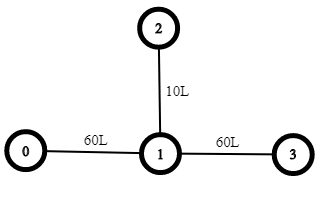
\includegraphics[width=1\linewidth]{img/graph_intro.png}
   \end{minipage}\hfill
\end{figure}
\end{center}

\indent Supongamos que en este caso los costos de combustible para las ciudades 0, 1, 2 y 3 son respectivamente 1, 50, 10, 50. Veamos las distancias de 0 a todos los demas. En primer lugar, tenemos una única forma de llegar al nodo 1, cargando 60L en un total de 60\$. Luego, la distancia de 0 a 1 es 60. Una vez que estamos en 1, tenemos dos opciones. Podemos cargar 10L e ir a 2 (por 500\$), o cargar 60 e ir a 3 (por 3000\$). Notemos que esta no es la mejor estrategia para llegar a 3, ya que podríamos ir a 2, cargar 60L, volver a 1, cargar 10L y de ahí pasar a 3 (por 1600\$). Esto nos resulta en costos totales de 60\$, 560\$ y 1660\$. \\
\indent Sin embargo, notemos que el camino de 0 a 3 resulta ser un camino no simple, lo que imposibilita la utilización de algunos algoritmos de camino mínimo, como Dijkstra. Por este motivo es que la transformación al grafo con 61*n nodos resulta de utilidad, ya que allí, este camino se vuelve simple. Nos permite estar en una misma ciudad más de una vez, pero el estado del tanque será distinto.

\clearpage

\section{Desarrollo}

\subsection{Transformación del grafo original}
Para resolver el problema planteamos la siguiente modificación del grafo original: cada ciudad c, antes representada por un único nodo, será ahora representada por 61 nodos distintos. Llamemos a cada uno de estos nodos $c_{i}$, con $0\leq i \leq 60$. Cada uno de estos significa ''estoy en la ciudad c con i litros de nafta en mi tanque''. \\
\indent En cuanto a las aristas, las dividiremos en dos grupos:
\begin{itemize}
\item Tipo A:  Las que van de un  $c_{i}$ a  $c_{i+1}$. Estas van a tener como peso el costo de cargar un litro de nafta en la ciudad c.
\item Tipo B: Las que van de una ciudad a otra. Estas aristas tendrán peso cero ya que al viajar no gasto dinero. Dos nodos $c_{i}$, $c'_{j}$, estarán conectados si y sólo si existe una ruta de $c$ a $c'$ con distancia $i-j$.
\end{itemize}

\indent Veamos que hallar un camino mínimo en el grafo, es equivalente a hallar una solución de nuestro problema. \\
\indent Comencemos por ver que existe una biyección entre los caminos de ambos grafos.\\ \\
\indent  \textbf{\underline{Demostración}:} Llamemos $G$ al grafo original y $G'$ al modificado. Y llamemos $s$ al vértice de salida, y $d$ al vértice de destino.\\
\indent Veamos primero que todo camino del grafo original está en el grafo modificado. \\
\indent Sea $C$ un camino de $s$ a $d$ en $G$. Construyamos un camino $C'$ en $G'$ que represente unívocamente a $C$. Supongamos que estoy en el i-ésimo vértice del camino, $v_{i}$. Ahora, si en $C$ cargamos $k_{i}$ litros de nafta en $v_{i}$ entonces vamos a tener $k_{i}$ aristas de tipo A moviéndose entre los distintos nodos que representan a $v_{i}$ en $C'$. Notemos que esta elección es única, pues estando en una ciudad con l litros, solo puedo cargar un litro de nafta, y hay una única arista que representa esta transición. Luego, cuando pasemos de $v_{i}$ a $v_{i+1}$, le vamos a agregar a $C'$ una arista de tipo B entre  $v_{i}$ y $v_{i+1}$. Esta arista también es única, ya que ir de una ciudad a otra tiene un costo fijo. Luego, si repetimos este proceso para cada $v_{i}$ en C, obtenemos el $C'$ que buscábamos. \\
\indent Ahora notemos que si tomamos un camino $C'$ en $G'$, las aristas de tipo A representan cuánta nafta cargo en un camino del grafo G, y las aristas de tipo B representan el movimiento entre ciudades. Sabiendo esto, la construcción del camino $C$ en $G$ resulta análogo. \\ %HACER GRAFO !!!!!!!!!!!!!!!!!!!!!!!!!!!
\indent Luego, si realizamos un algoritmo de caminos mínimos sobre el grafo modificado, el costo mínimo encontrado coincide con el costo mínimo del grafo original, que es la respuesta al problema que queríamos resolver.

\subsection{Dijkstra}
Utilizaremos Dijkstra para calcular distancia mínima de un nodo a todos sus vecinos. Algunas particularidades de Dijkstra son:
\begin{enumerate}
\item Dijkstra tiene como precondición que no haya ejes de peso negativo, lo cual nuestro problema garantiza.
\item Es similar al algoritmo de Prim, pero generalizado para una función $c_{\bullet}$ creciente.
\item Si tomamos la función $c_{+}$ este algoritmo resuelve el problema de camino mínimo desde un nodo a los demás.
\end{enumerate}

\indent El pseudocódigo de Dijkstra\footnote{fuente: teórica.} es el siguiente:
\begin{algorithm}[H]
\caption{Dijkstra$\bullet$}
\label{$Dijkstra$}
\begin{algorithmic}[1]
\Procedure{$Dijkstra_{\bullet}$}{grafo $G$, nodo $salida$, funcion $c_{\bullet}$}
\State $res$ $\gets$ crearVectorDeTama\~noConValor(cantNodos, indefinido)
\State $res[salida] \gets$ elementoNeutro($c_{\bullet}$)
\For{$i$=1,...,cantNodos-1}
\State $(x,y) \gets$ arista segura de G con mínimo $c_{\bullet}(xy)$  \Comment{Consideramos $x$ ya definido, $y$ no definido.}
\State $res[y] \gets c_{\bullet}(x,y)$
\EndFor
\State return $res$
\EndProcedure
\end{algorithmic}
\end{algorithm}

\indent En particular para la función $c_{+}$:
\begin{algorithm}[H]
\caption{Dijkstra+}
\label{$Dijkstra$}
\begin{algorithmic}[1]
\Procedure{$Dijkstra_{+}$}{grafo $G$, nodo $salida$}
\State $res$ $\gets$ crearVectorDeTama\~noConValor(cantNodos, indefinido)
\State $res[salida] \gets$ 0
\For{$i$=1,...,cantNodos-1}
\State $(x,y) \gets$ arista segura de G con mínimo $c_{+}(xy)$ \Comment{Consideramos $x$ ya definido, $y$ no definido.}
\State $res[y] \gets c_{+}(x,y)$						\Comment{res[$y$] = res[$x$]+peso($xy$)}
\EndFor
\State return $res$
\EndProcedure
\end{algorithmic}
\end{algorithm}

\indent Complejidad\footnote{fuente: clases teóricas.}: \\ \\
\indent Sea $n$ la cantidad de vértices, y $m$ la cantidad de aristas:
\begin{itemize}
\item Caso ralo: usar una cola de prioridad sobre heap con todas las aristas seguras. Costo $T(n + m) =  \mathcal{O}(mlgn)$
\item Caso general: usar diccionario de costo que contenga el valor de la mejor arista segura para cada $y \notin  V (T)$. Costo $T(n + m) = \mathcal{O}(m+nlgn)$.
\item Caso denso: implementar el diccionario de costos sobre un vector. Costo $T(n + m) = \mathcal{O}(n^{2}).$
\end{itemize}

\indent La implementación fue extraída de internet\footnote{fuente: https://www.geeksforgeeks.org/dijkstras-shortest-path-algorithm-greedy-algo-7/} y modificada para adaptarla a nuestras estructuras. Como fue implementado sobre vector la complejidad es $\mathcal{O}(n^{2})$. \\

\indent Notemos que Dijkstra nos devuelve el camino mínimo de un vértice hacia todos sus vecinos. Trasladado a nuestro problema, esto nos daría el costo mínimo de combustible que necesitamos para partir de una ciudad y llegar a cualquier otra. Sin embargo el problema nos pide saber esto mismo pero partiendo de cualquier ciudad. Es por esto que debemos llamar a Dijkstra una vez por nodo, es decir llamamos a Dijkstra n veces, lo cual transforma nuestra complejidad en $\mathcal{O}(n^{2})$. \\
\indent Sin embargo, nos faltan analizar unos detalles más, ya que no corremos el algoritmo sobre el grafo original, sino sobre una modificación. \\
\indent En primer lugar la cantidad de nodos del grafo aumenta. Si la cantidad de ciudades era $n$, la cantidad de nodos del grafo modificado será $61*n$. Pero como 61 es una constante, las complejidades teóricas no se modifican, sin embargo en la práctica la diferencia entre correr Dijkstra con $n$ nodos, y con $61*n$ nodos, puede ser notoria.\\
\indent Algo similar sucede con la cantidad de aristas. Dada una ruta del grafo original, como mucho se va a replicar 120 veces. Esto sucede cuando la arista tiene costo 1L, entonces voy de $a_{60}\rightarrow b_{59}$, ....$a_{1} \rightarrow b_{0}$ y viceversa. Además, se agrega una cantidad fija de 60*n aristas, las de tipo A. Sin embargo, como asumimos que el grafo es conexo, n=O(m). Luego la cantidad de aristas en el grafo modificado es $\mathcal{O}(cantidadDeRutas)$, por lo tanto esto tampoco afecta la complejidad teórica. \\
\indent Finalmente tiene sentido preguntarnos sobre qué nodo empezamos y sobre cuál terminamos, ya que antes cada nodo represtaba una única ciudad, y en el nuevo grafo, hay 61 nodos que representan la misma ciudad. La respuesta es que por cada ciudad $c$ nos interesa salir de un solo nodo, el que representa estar en la ciudad $c$ con 0 litros de nafta. Por esta razón, solo es necesario llamar a Dijkstra, $cantidadDeCiudades$ veces\footnote{Por esta razón, en main.cpp el for aumenta de a 61.}. Además en cuanto a los nodos de llegada solo nos interesa el caso de llegar con 0 litros, ya que en otro caso habríamos cargado nafta de más y sería subóptimo.

\subsection{Dijkstra con cola de prioridad}
Este algoritmo tiene el mismo pseudocódigo que la sección anterior. Es Dijkstra con una implementación particular de cola de prioridad. Por esta razón, como expusimos anteriormente, la complejidad teórica de cada llamado es $\mathcal{O}(mlgn)$. \\
\indent También como en el algoritmo, anterior lo llamamos n veces para computar los caminos mínimos de cada vértice hacia todos los demás. Luego la complejidad total es $\mathcal{O}(nmlgn)$.

\subsection{Bellman-Ford}
Al igual que Dijkstra, Bellman-Ford calcula los caminos mínimos desde un vértice a todos los otros.\\
\indent Su complejidad temporal es $\mathcal{O}(mn)$, y la espacial $\mathcal{O}(n+m)$. \\
\indent Pseudocódigo del algoritmo\footnote{fuente: teórica.}:

\begin{algorithm}[H]
\caption{Bellman-Ford}
\label{$BF$}
\begin{algorithmic}[1]
\Procedure{$Bellman-Ford$}{grafo $G$, nodo $salida$}
\State Crear un diccionario $D^{0}$ con $D^{0}[salida]$ = 0 y $D^{0}[y]$ = $\infty$, y $\neq$ v
\For{$i$=1,...,cantNodos-1}
\State Crear un diccionario $D^{i-1}[y]$ = mín\{ $D^{i}[x]$ + peso(xy) / $x \in N^{in}[y]$ \} $\forall$ $y \in V(G)$.
\EndFor
\State return $D^{n-1}$
\EndProcedure
\end{algorithmic}
\end{algorithm}

\indent Por lo mismo que en Dijkstra, hacemos cantidadDeCiudades llamados a Bellman-Ford, y la complejidad teórica es $\mathcal{O}(mn^{2})$, con n la cantidad de ciudades y m la cantidad de rutas.

\subsection{Floyd-Warshall}
Este algoritmo se diferencia de los anteriores en que en vez de calcular las distancias mínimas de un vértice hacia los otros, calcula las de todos los vértices hacia todos los otros. Por esta razón, no hay que llamarlo más de una vez.\\
\indent La complejidad de este algoritmo es $\mathcal{O}(n^3)$. Sin embargo, hay que notar que n no es la cantidadDeCiudades, sino que es 61*cantidadDeCiudades. Aunque la complejidad teórica no cambie, esto puede tener un impacto en el tiempo de ejecución en la práctica. Notemos además que en los algoritmos anteriores hacemos $cantidadDeciudades$ llamados, salteando otros 60 nodos por ciudad que no nos interesan para resolver el problema. Al llamar a Floyd-Warshall una única vez, estos $60*cantidadDeCiudades$ problemas que habíamos salteado, se resuelven.

\begin{comment}
El input de nuestro problema consiste en un grafo completo $G=(V,E)$ con pesos en las aristas $d: E \rightarrow N$, y un valor de nafta $c: V \rightarrow N$, y una capacidad de tanque $U$. Equivalentemente, si no nos es dado un grafo completo, podemos definir $d_{uv}$ como la distancia entre u y v en G. Nuestro objetivo es ir desde un comienzo s hacia un destino t de la forma mas barata posible. Para una fácil exposición nos concentramos en el caso en que comenzamos en s con el tanque vacío. Para el caso en que comenzamos con $\delta_{s}$ unidades de nafta, el mismo puede ser reducido de la siguiente manera: Agregamos un nuevos nodo $s_{0}$ tal que $d_{s_{0}s} = U - \delta_{s}$ y $c(s_{0}) = 0$. El problema de empezar en s con $\delta_{s}$ unidades de nafta y de empezar en $s_{0}$ con el tanque vacío usando una parada adicional, es equivalente.

Resolveremos el problema presentado utilizando la siguiente formulación basada en programación dinámica (PD):
\begin{equation*}
	D[u, g] = \text{Minimo costo de ir desde u hasta t, empezando con g unidades de nafta.}
\end{equation*}


\begin{lemma}
Sea $s = u_{1}, u_{2}, ... , u_{l}$ las paradas de recarga de una solución óptima utilizando como máximo $\Delta$ paradas.
La siguiente es una estrategia óptima para decidir la cantidad de gas que se va a llenar en cada parada:
en la parada $u_{l}$ cargamos nafta suficiente para alcanzar t con el tanque vacío; para $j <l$:
\begin{enumerate}
 	\item Si $c(u_{j}) < c(u_{j+1})$, entonces en $u_{j}$ llenamos el tanque.
 	\item Si $c(u_{j}) \geq c(u_{j+1})$, entonces en $u_{j}$ llenamos lo suficiente para llegar a $u_{j+1}$
\end{enumerate}
\end{lemma}

\textbf{\underline{Demostración:}} Si $c(u_{j}) < c(u_{j+1})$ y en la solución optima no llenamos en $u_{j}$ luego podemos incrementar la cantidad cargada en $u_{j}$ y decrementar la cantidad en $u_{j+1}$. Esto mejoraría el costo total de la solución, lo que contradice que habíamos asumido que teníamos una solución optima. Similarmente, si $c(u_{j}) \geq c(u_{j+1})$ luego podemos decrementar la cantidad de nafta cargada en $u_{j}$ e incrementar la cantidad cargada en $u_{j+1}$ (sin incrementar el costo total de la solución) hasta que se cumpla la condición.

Consideremos una parada de recarga $u \neq s$ en la solución óptima, y sea $w$ la parada justo antes de u.
El lema 1 implica que si $c(w) > c(u)$, alcanzamos u con un tanque vacío, de lo contrario alcanzamos u con $U - d(w, u)$ de nafta. Por lo tanto, en nuestra formulación de PD debemos seguir al menos n diferentes valores de gas para $u$. Sea $GV(u)$ el conjunto de tales valores, a saber:

\begin{equation*}
GV(u) = \lbrace U - d(w, u)| \ w \in V \ y \ c(w) < c(u) \ y \ d(w, u) \leq U\rbrace u \lbrace 0 \rbrace
\end{equation*}

Volviendo a nuestra formulación de programación dinámica:
Claramente, $D(t, 0) = 0$. Para otros vértices $u \neq t$ y $g \in GV(u)$, los valores óptimos obedecen la siguiente recurrencia:

\[
D(u,g) = min
	\begin{cases}
		D(v, 0) + (d_{uv} - g) c(u) 		& \text{si $c(v) \leq c(u) \vee v = t$ y $g \leq d_{uv}$ } \\
		D(v, U - d_{uv}) + (U - g) c(u) 	& \text{si $c(v) > c(u)$}
	\end{cases}
\]

Presentamos el siguiente ejemplo:

\begin{figure}[h]
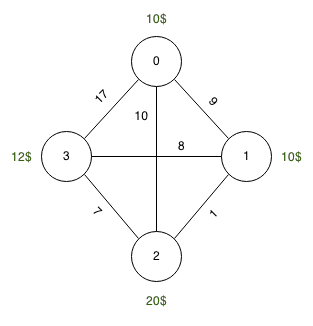
\includegraphics[width=8cm]{ex}
\centering
\end{figure}

siendo los cálculos finales:


$GV[0] = \lbrace 0 \rbrace, \ \ GV[1] = \lbrace 0 \rbrace, \ \ GV[2] = \lbrace 0, 3, 9 \rbrace, \ \ GV[3] = \lbrace 0, 2 \rbrace$


$D(0,0) = min \lbrace D(1,0) + 9 * 10 \rbrace$


$D(1,0) = min \lbrace D(2,9) + 10 * 10, D(3,0) + 8*10 \rbrace$


$D(3,0) = 0$


y asi siguiendo...

por lo tanto $D(0,0) = 170$
\end{comment}

\clearpage

\section{Implementaci\'on}
En esta sección explicaremos las estructuras elegidas para representar los datos.

\subsection{Arco}
Para representar los ejes de un grafo creamos la struct arco, con los siguientes atributos:
\begin{itemize}
\item peso
\item cola
\item cabeza
\end{itemize}
Si tenemos una arista m que va de un nodo $a$, a un nodo $b$ con un valor $k$. Luego podemos representar m de la siguiente forma:
\begin{itemize}
\item peso = k
\item cola = a
\item cabeza = b
\end{itemize}

\subsection{Grafo}
Para representar grafos elegimos una representación basada en lista de adyacencias. Para esto, creamos la estructura grafoAd con los siguientes atributos:
\begin{itemize}
\item listaAd: es un vector de listas. Cada posición $i$ del vector guarda una lista con los arcos salientes del nodo $i$. Es decir, guarda los vecinos a los que se puede acceder desde $i$, con el peso de la arista que lo permite\footnote{Además por ser eje guarda la cola de la arista, que en este caso será $i$ para todos los ejes de la lista.}.
\item cantNodos: es un entero que guarda la cantidad de nodos del grafo.
\item cantAristas: es un entero que guarda la cantidad total de aristas del grafo.
\end{itemize}

\indent Y los siguientes métodos:
\begin{itemize}
\item grafoAd: es el constructor de la clase. Inicializa cantNodos y cantAristas en cero, y la lista de adyacencias como un vector vacío.
\item agregarNodo: agrega una nueva posición al vector, con una lista vacía.
\item agregarEje: agrega una arista al grafo, con el peso y los nodos especificados en los parámetros.
\end{itemize}

\newpage

\subsection{Lectura de la entrada}

A partir de la entrada del programa, generamos el grafo modificado. Para lograrlo, generamos un grafo con n'=61*n nodos, donde el nodo i representa al nodo i/61 del grafo original, en un estado con i mod 61 Litros de nafta. Por ejemplo, si teníamos un grafo con 100 nodos, en el grafo modificado el nodo 176 representa a la ciudad 2 con 54 litros en el tanque. \\
\indent Sabiendo esto, para cada costo $C_{i}$ de combustible leido generamos 61 vertices, donde cada uno está unido al siguiente con una arista de costo $C_{i}$. De esta manera, logramos generar todas las aristas de tipo A. \\
\indent Por último, para cada ruta leida, generamos las aristas de tipo B. Si una ruta es representada con los enteros $a_{i}$, $b_{i}$, $l_{i}$ (ambas ciudades seguidas del costo de la ruta), vamos a decir que una arista representa un movimiento valido si $a_{i}$ representa un estado con $K$ litros en el tanque, y $b_{i}$ representa un estado con $k$-$l_{i}$ litros. Luego, simplemente debemos conectar un nodo de la ciudad $a_{i}$ a otro de $b_{i}$ (y viceversa) si representan un movimiento valido. \\
\indent Presentamos el pseudocodigo a continuación:

\begin{algorithm}[H]
\caption{crear grafo modificado}
\label{img2sorted}
\begin{algorithmic}[1]
\Procedure{crearGrafoModificado}{}
\State $i \gets 0$
\For{$i < cantidadDeCiudades$}
	\State G.agregarNodo()
	\State $j \gets 1$
	\State precioNafta $\gets$ precioNaftaEn(i)
	\For{$j < 61$} \Comment{Generamos aristas de tipo A}
		\State G.agregarNodo()			\Comment{El nodo de estar en la ciudad i con j litros}
		\State a $\gets 61*i+j-1$			\Comment{Tener j-1 litros en la ciudad i}
		\State b $\gets$ siguienteDe(a)		\Comment{Tener j litros en la ciudad i}
		\State G.agregarEje(precioNafta, a, b) \Comment{Costo de pasar de tener j-1 litros, a tener j en la ciudad i}
	\EndFor
\EndFor

\State $i \gets 0$
\For{$i < cantidadDeRutas$}
	\State a $\gets$ extremoADeArista(i)
	\State b $\gets$ extremoBDeArista(i)
	\State l $\gets$ cantidadDeLitrosDeAaB(i)
	\State j $\gets$ 0
	\For{j $<$ 61} 					\Comment{Generamos aristas de tipo B}
		\If{j-l $\geq$ 0} 				\Comment{Si puedo ir de a a b con la nafta que tengo}
			\State a' $\gets$ a*61+j
			\State b' $\gets$ b*61+j-l
			\State G.agregarEje(0, a', b') 	\Comment{La arista de viajar de la ciudad a a b con l litros de nafta}
			\State a' $\gets$ a*61+j-l
			\State b' $\gets$ b*61
			\State G.agregarEje(0, b', a')	 \Comment{La arista de viajar de la ciudad b a a con l litros de nafta}
		\EndIf
	\EndFor
\EndFor
\State return G
\EndProcedure
\end{algorithmic}
\end{algorithm}

\indent Complejidad: $\mathcal{O}(n+m)$

\subsection{Impresión por salida estándar}
Para imprimir el resultado, simplemente hay que ser cuidadosos y recordar que nuestro nuevo grafo contiene nodos que no nos interesan (Solo queremos empezar y terminar en estados en los que tenemos 0 Litros en el tanque). De esta forma, si terminamos con una matriz de distancias, solo debemos imprimir aquellas posiciones cuyas columnas o filas sean iguales a 0 modulo 61.

%\begin{algorithm}[H]
%\caption{imprimir resultados del programa}
%\label{}
%\begin{algorithmic}[1]
%\Procedure{imprimirResultado}{$matriz$ distancias}
%\State i $\gets$ 0
%\For{i$<$distancias.size()}
%	\State j $\gets$ 0
%	\For{j$<$distancias.size()}
%		\If{i $\neq$ j}
%			\State imprimir(i, j, distancias$[i][j]$) \Comment{Imprimir la mínima distancia de ir de i a j}
%		\EndIf
%	\EndFor
%\EndFor
%\EndProcedure
%\end{algorithmic}
%\end{algorithm}
%
%\indent Complejidad: $\mathcal{O}()$

\clearpage

\section{Experimentación}
A continuaci\'on analizaremos los distintos aspectos de la resoluci\'on implementada para la segmentaci\'on. Debido a las características del problema, la discusi\'on se centrar\'a en dos ejes principales: como esta es una implementaci\'on particular debemos considerar su eficiencia y las propiedades que posee midiendo las métricas correspondientes. Por otro lado, como se present\'o en la introducci\'on, este problema carece de una respuesta objetiva y absoluta, por lo tanto se buscar\'a dar cierto parámetro del objetivo buscado y responder si el algoritmo lo satisface. \\
\indent Específicamente los experimentos realizados consisten en comparar el efecto que tienen las distintas estructuras planteadas en la secci\'on de desarrollo y justificar la complejidad temporal propuesta. Luego analizaremos si la funci\'on de \textit{threshold} planteada en \cite{Felzenszwalb2004} cumple la propiedad propuesta. Hechas estas consideraciones buscaremos dar una respuesta a cu\'al es la calidad de la segmentaci\'on utilizando un \textit{dataset} con su correspondiente \textit{groundtruth}. Por último veremos c\'omo se comporta el algoritmo frente a distintas posibles aplicaciones y se intentara determinar si es apto para alguna de ellas.      

\subsection{Comparaci\'on de las estructuras}
Como se explic\'o en la secci\'on de implementaci\'on, para realizar ciertas operaciones en el algoritmo\ref{segmentation}, es necesario utilizar un tipo abstracto de datos \textit{Disjoint Set}. Se mostr\'o que este pod\'ia ser implementado de al menos tres formas distintas y se justificaron las complejidades. Ahora vamos a evaluar cuál es el rendimiento del algoritmo utilizando las distintas estructuras posibles.\\
\indent Para este experimento se tom\'o una imagen original de dimensiones de $1240\times 960$ píxeles a la cual se la redimension\'o a distintos tama\~nos. Luego se ejecut\'o el algoritmo para cada imagen y se midi\'o el tiempo en realizar únicamente la segmentaci\'on, ya que se consider\'o que la lectura de la imagen y la generaci\'on de las aristas era constante para las tres versiones. Además para este experimento se considera que tanto el contenido de la imagen original como el valor de $k$ es irrelevante al tiempo que toma la ejecuci\'on.\\
\indent Basado en lo discutido sobre el an\'alisis te\'orico del costo, se esper\'o que la estructura que tarde m\'as tiempo sea el arreglo de representantes, seguido del arbol de representantes y luego la versi\'on con \textit{path relinking}. Esto se justifica en el hecho de que los \textit{unite} del arreglo tardan estrictamente $n$ pasos, mientras que en este contexto para los arboles de representantes esta operaci\'on se realiza en tiempo constante. Además el uso de \textit{path relinking} tiene un costo te\'orico menor al de las otras dos opciones, por lo tanto explicar\'ia que sea la versi\'on optima respecto al resto.
\vspace{-3mm}
\begin{figure}[H]
\begin{center}
	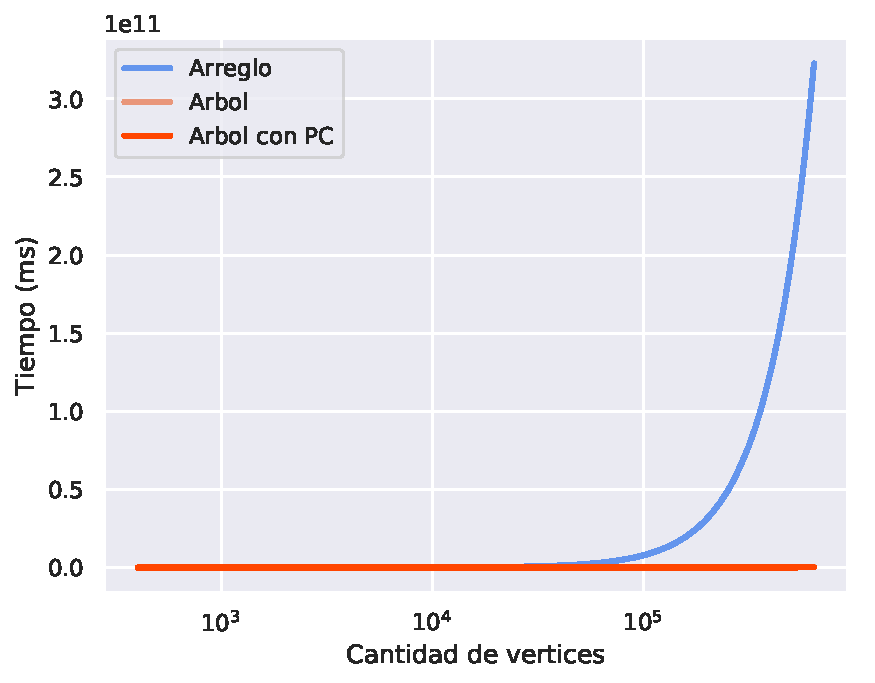
\includegraphics[scale=0.5]{plots/compEstr.pdf}
	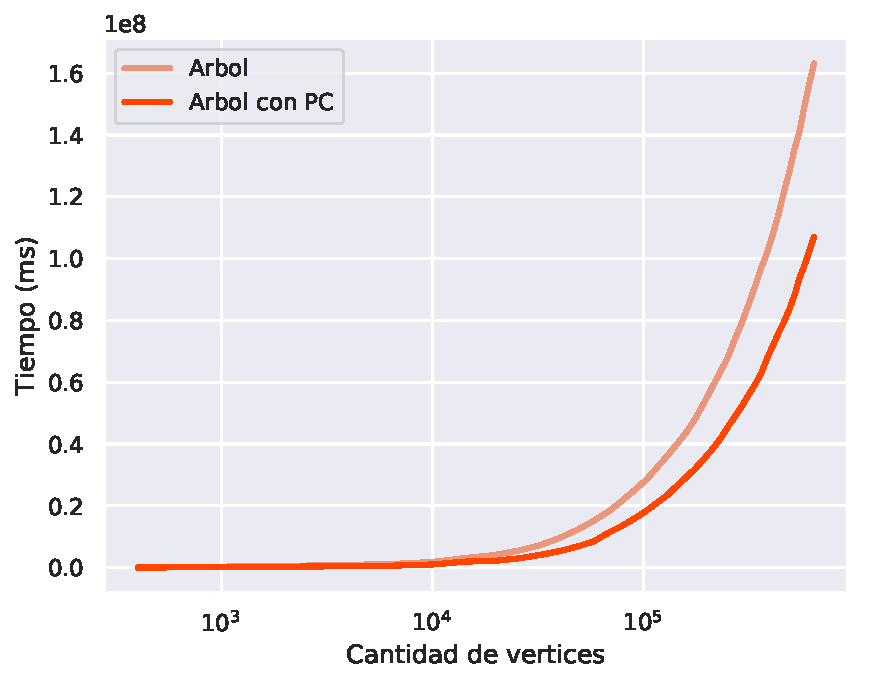
\includegraphics[scale=0.5]{plots/comp_arbs.pdf}
	\caption{Comparaci\'on de tiempos para las distintas estructuras. La cantidad de vértices es de $(20p)^2$ con $p\in[1,40]$ y $k=1000$.}
	\label{comp_estr}
\end{center}
\end{figure}
\vspace{-7mm}

\indent Efectivamente se cumpli\'o experimentalmente lo que se esperaba en base al costo te\'orico. Podemos ver como el ritmo de crecimiento que conlleva utilizar el arreglo de representantes supera vastamente al de los árboles, debido a esto es necesario visualizar por separado el rendimiento de las estructuras de árboles. En el segundo gr\'afico se ve como para instancias de tama\~no mayor sí aparenta haber una notable diferencia entre las opciones, sin embargo no parecer\'ia que utilizar árbol de representaci\'on tenga un ritmo de crecimiento muy distinto a la versi\'on con \textit{path relinking}, sino más bien que hay una diferencia en la constante de multiplicaci\'on. Un experimento posible que no se realiz\'o es comprobar si en la práctica y para esta aplicaci\'on usar un árbol de representantes implica un costo lineal del algoritmo. Esto último no se comprob\'o ya que, aunque llegue a ser cierto, sigue siendo conveniente utilizar \textit{path relinking}.

\subsubsection{An\'alisis temporal del algoritmo}
Habiendo hecho la comparaci\'on en el experimento anterior y habiendo decidido que utilizar \textit{path relinking} era ventajoso, se propuso medir el tiempo de la totalidad del procedimiento esta vez teniendo en cuenta el costo de conseguir el grafo a partir de la imagen. Esto resulta de interés ya que al fin y al cabo el procedimiento en su totalidad es lo que verdaderamente se quiere saber si es eficiente o no. Para esto se tomó el mismo conjunto de im\'agenes propuesto para el experimento anterior y el mismo valor de $k$. El objetivo es mostrar empíricamente que el costo total de todo el algoritmo es de $\mathcal{O}(n)$. \\
\indent Con fines de justificar esta afirmaci\'on se utiliz\'o la teor\'ia de \textit{cuadrados m\'inimos lineales}:\\
\indent Poseemos una muestra de valores de tiempo en funci\'on del tama\~no de entrada $(n_1, t_1) \dots (n_k, t_k)$ y queremos aproximarlos con una funci\'on $f \in F$ familia de funciones, de forma que $f$ minimice la expresión: 
\[
	\sum_{i=1}^k(f(n_i)-t_i)^2
\]
Esta teor\'ia nos es útil pues podemos tomar la familia de funciones $F: \ an+b$. Luego la teor\'ia nos asegura que siempre podemos determinar los coeficientes $a$ y $b$ que minimizan la expresi\'on. Esto nos es ventajoso pues de esta forma encontramos una funci\'on que pertenece al supuesto orden del peor caso de nuestro algoritmo y que además minimiza el criterio de cuadrados m\'inimos.  
Luego de haber conseguido estos coeficientes (y por lo tanto la funci\'on) podemos utilizar la \textit{fórmula de Pearson} sobre las muestras $(n_1, t_1) \dots (n_k, t_k)$ y $(n_1, f(t_1)) \dots (n_k, f(t_k))$ y as\'i obtener una m\'etrica sobre el grado de correlaci\'on entre los datos y la funci\'on. 
\begin{figure}[H]
	\begin{center}
		\subfigure[Comparaci\'on de tiempo de ejecuci\'on y costo te\'orico]{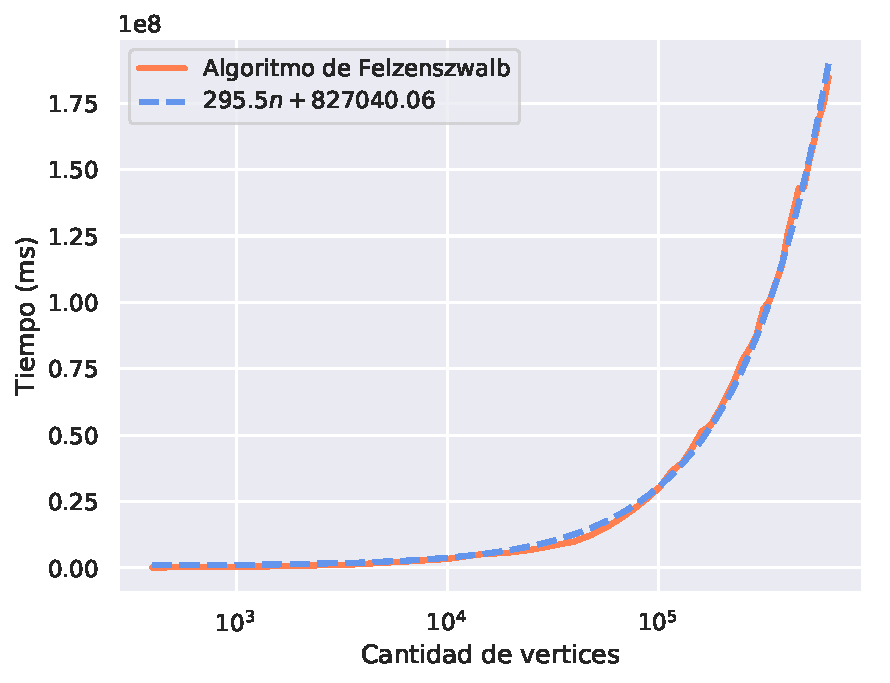
\includegraphics[scale=0.5]{plots/tiempo_Felzen.pdf}}
		\subfigure[Correlaci\'on entre el algoritmo y el costo te\'orico]{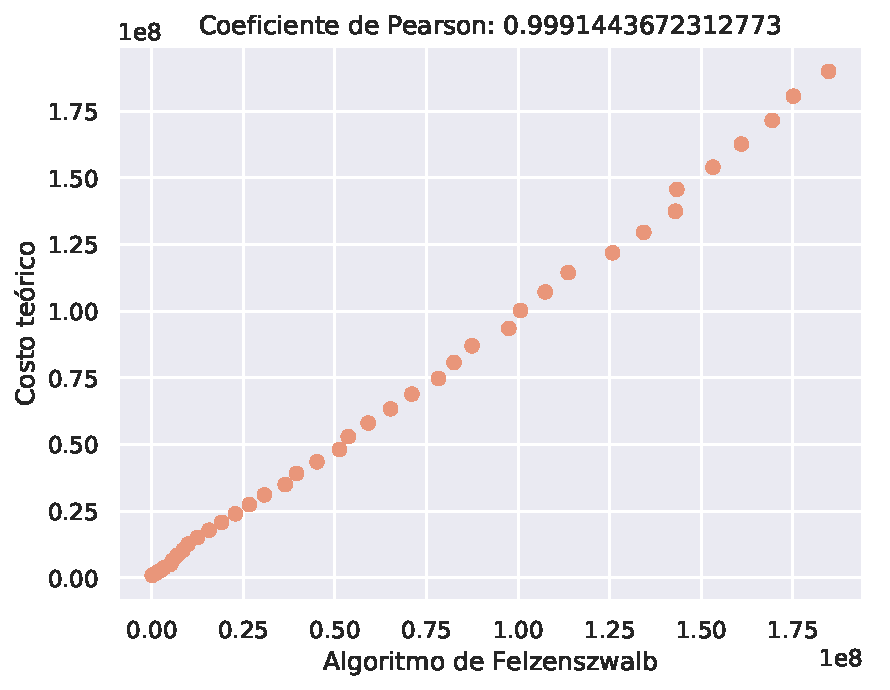
\includegraphics[scale=0.5]{plots/Felzen_corr.pdf}}
		\label{costo_teo}
	\end{center}
	\caption{}
\end{figure}
\vspace{-7mm} 

\indent Como era esperado los datos obtenidos soportan la complejidad te\'orica propuesta, dejando en claro que el algoritmo implementado es eficiente para el problema a resolver. 


\subsection{Influencia de $k$ sobre la granularidad del resultado}
En el trabajo \cite{Felzenszwalb2004} se toma la funci\'on de \textit{threshold} $\tau(C)=\frac{k}{\#C}$ con $k$ un hiperparámetro. Intuitivamente podemos ver que un $k$ menor da lugar a componentes más chicas y análogamente un $k$ mayor tiende a unir componentes, ya que afecta directamente sobre el predicado que da evidencia si hay un l\'imite entre componentes. El objetivo del siguiente experimento es buscar una correlaci\'on empirica entre esta noci\'on y las segmentaciones resultantes. \\
Para poder dar una afirmaci\'on estadisticamente robusta se utiliz\'o el \textit{Berkeley Segmentation Dataset} (BSDS) \cite{BSDS} que consiste en 300 im\'agenes variadas. Luego se comput\'o la segmentaci\'on para cada valor de $k$ y para cada imagen, midiendos\'e la cantidad de componentes distintas. 

\begin{figure}[H]
	\begin{center}
	\subfigure[Imagen de ejemplo perteneciente al BSDS]{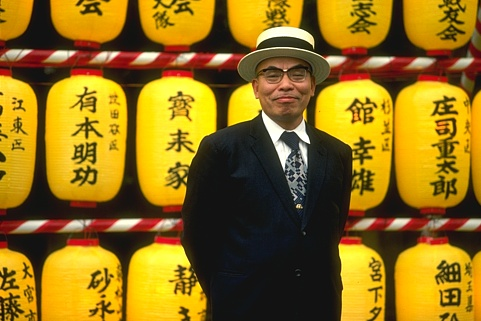
\includegraphics[scale=0.35]{segmentaciones/sr.jpg}}
	\hspace{5mm}
	\subfigure[Cantidad de componentes para distintos $k$]{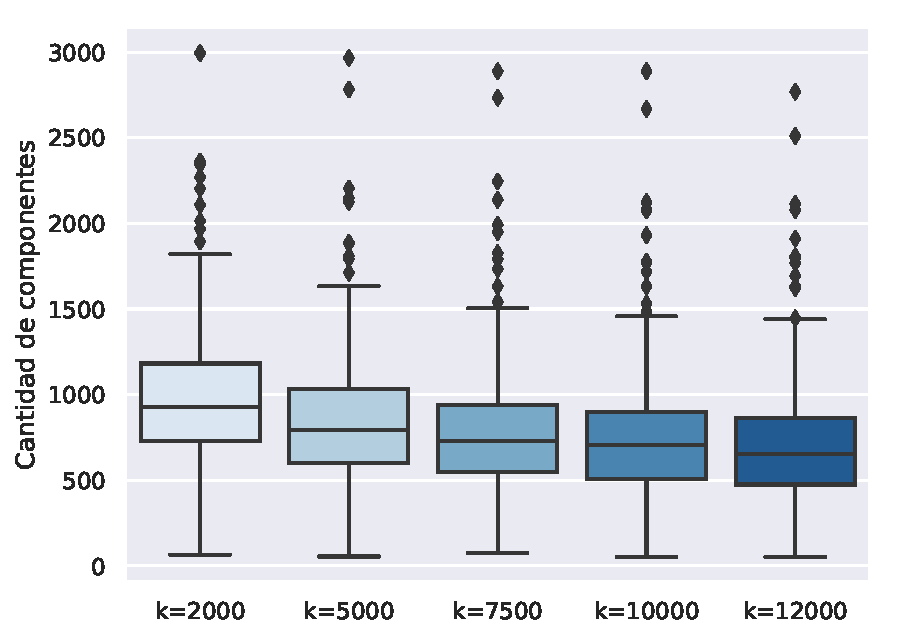
\includegraphics[scale=0.5]{plots/boxplot_k.pdf}}
	\caption{}
	\end{center}
	\label{comp_k}
\end{figure}
\vspace{-7mm} 

\indent Como podemos observar en la figura 4 \textit{(b)}, a medida que se aumenta el $k$ la media de componentes disminuye. Además las relaciones de los cuartiles no son afectadas, lo que lleva a pensar que para todas las imagenes la influencia del valor de $k$ afecta de manera similar.

\begin{figure}[H]
	\begin{center}
	\subfigure[$k=2000$]{
\includegraphics[scale=0.35]{segmentaciones/sr-2000.jpg}}
	\hspace{1mm}
	\subfigure[$k=5000$]{
\includegraphics[scale=0.35]{segmentaciones/sr-5000.jpg}}
	\hspace{1mm}
	\subfigure[$k=7500$]{
\includegraphics[scale=0.35]{segmentaciones/sr-7500.jpg}}
	\hspace{1mm}
	\subfigure[$k=10000$]{
\includegraphics[scale=0.35]{segmentaciones/sr-10000.jpg}}
	\hspace{1mm}
	\subfigure[$k=12000$]{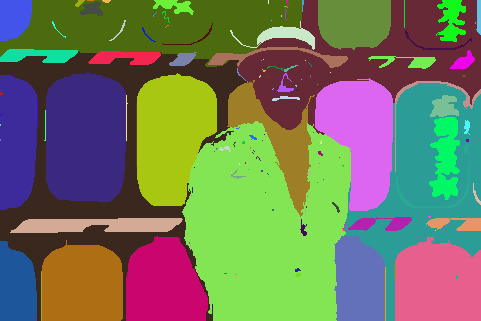
\includegraphics[scale=0.35]{segmentaciones/sr-12000.jpg}}
	\caption{}
	\end{center}
	\label{costo_teo}
\end{figure}
\vspace{-7mm} 

\indent En la foto usada de ejemplo podemos ver efectivamente el efecto de incrementar al hiperparámetro. En un principio los rasgos faciales son m\'as faciles de distinguir y los kanjis en las linternas no fueron todav\'ia considerados como el interior del objeto. Al mismo tiempo se ve mucha variabilidad en zonas que se esperar\'ian uniformes como el saco. A medida que se incrementa el valor vemos como se alisan ciertas secciones, ganando mayor definici\'on y separaci\'on pero algunos detalles como los ideogramas se pierden. Ya para los últimos casos los contornos generales quedan mayormente separados con muy pocos detalles peque\~nos distinguibles. Notar que estas últimas generalizaciones a componentes m\'as grandes puede traer uniones no deseadas, como es el caso del cuello de la camisa en este ejemplo: para $k=5000$ hay una distinci\'on con la lampara que interseca con la camisa, pero para todos los valores de $k$ siguientes estas dos regiones se unen.\\
\indent Este experimento confirma la intuici\'on original sobre los efectos del hiperparámetro $k$ y se tendrán en cuenta para la experimentaci\'on siguiente.


\subsection{Calidad de la segmentaci\'on}
Si bien el objetivo de resolver el problema es dar una segmentaci\'on que refleje los objetos de interés en una imagen, como ya se mencion\'o, esto es completamente subjetivo. Principalmente hay dos partes fundamentales a esta subjetividad, una siendo que es lo que se quiere estudiar de un conjunto de imágenes (cual es el objeto de interés) y la otra respecta al observador de la imagen segmentada (quien aprueba el resultado). Aunque este sea el caso no quita que sea de interés poder dar una respuesta a la pregunta de cu\'an buena es una segmentaci\'on. \\
\indent Con este objetivo se consider\'o utilizar un \textit{data set} que posea la \textit{ground truth} de las segmentaciones: segmentaciones fabricadas por humanos que se consideraran como la respuesta objetivamente correcta al problema. Se utiliz\'o un subconjunto del BSDS presentado en \cite{li2013benchmark} en el cual se propone una construcci\'on del \textit{ground truth} basada en niveles de percepción de la imagen y consideran que su objeto de estudio son las figuras contrastantes con los distintos fondos de la imagen original. A grandes rasgos consideran que la segmentaci\'on debe ser gruesa y bien definida. \\
\indent A partir de este \textit{data set} se implement\'o una comparaci\'on entre las imágenes \textit{ground truth} y la segmentaci\'on obtenida. La m\'etrica considerada fue el $F_2$ score:
\[
	F_2 = (1+2^2)\frac{\text{Precision}\times{Recall}}{2^2\times \text{Precision}+\text{Recall}}
\]
\indent En este contexto \textit{Precision} significa saber de todos los píxeles que la segmentaci\'on clasifico en la misma componente, cuantos verdaderamente lo estaban. \textit{Recall} representa cuántas asociaciones correctas se hicieron. Por el problema a resolver y las consideraciones hechas en \cite{Felzenszwalb2004} se consider\'o darle mayor importancia al valor de \textit{Recall} para reforzar el peso de los \textit{falsos negativos}: poner un l\'imite entre dos componentes cuando no lo hay. Con esto se justifica usar $\beta =2$ para el $F_{\beta}$ score.\\
\indent Para cada píxel $P_i$ se consider\'o su \textit{k-ring} de píxeles $P_j$, comparando para cada par si pertenecían o no a la misma componente en la segmentaci\'on obtenida y en la \textit{ground truth}. Con esto se obtienen los valores de \textit{true positives, false positives, true negatives} y \textit{false negatives}. En la experimentaci\'on se consider\'o el \textit{5-ring}, con la justificaci\'on que este radio proporcionar\'ia suficiente informaci\'on local (contexto del píxel $i$). \\
\indent Como las componentes que se generan son de gran tama\~no, hacer el procedimiento para todo pixel desbalancear\'ia la cantidad de \textit{true positives}. Esto se debe a que se tendr\'ian en cuenta grandes porciones lisas de la imagen y estas no proporcionan gran informaci\'on sobre los puntos de interés (los l\'imites). Por lo tanto se tuvo en cuenta \'unicamente los píxeles ``borde'' de la segmentaci\'on obtenida. Esto mide mejor lo propuesto ya que si un píxel es de ``borde'' en la imagen obtenida pero no lo es en la \textit{ground truth} aumentarán los \textit{false positives} que es justamente lo que se considera importante de captar.

\begin{figure}[H]
	\begin{center}
	\subfigure[$F_2$ scores para el data set]{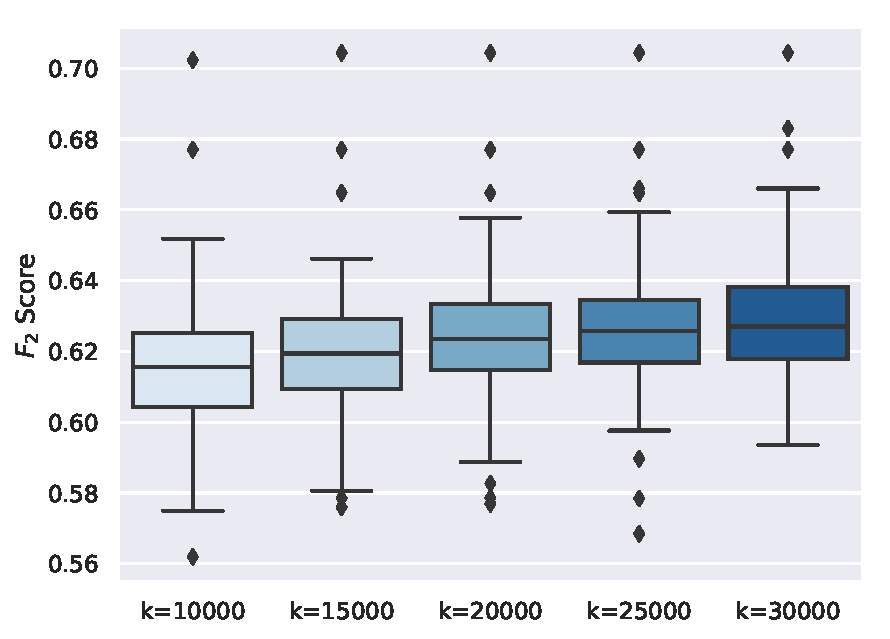
\includegraphics[scale=0.5]{plots/fScores_k.pdf}}
	\hspace{3mm}
	\subfigure[Desviaci\'on estandar de la m\'etrica]{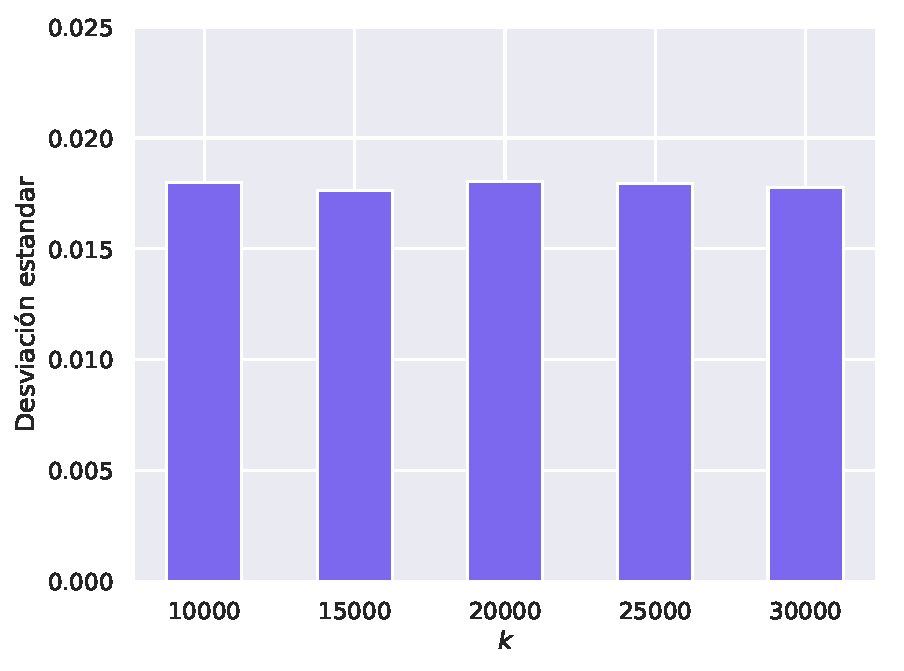
\includegraphics[scale=0.5]{plots/std_k.pdf}}
	\caption{}
	\end{center}
	\label{Fscores}
\end{figure}
\vspace{-7mm} 

\indent En primer lugar se observa que si bien hay una mejora en la calidad de segmentaci\'on a medida que se toma un $k$ mayor, este incremento es relativamente peque\~no ya que las medias de $k=10000$ y $k=30000$ difieren en no m\'as de $0.04$. A su vez, la variabilidad que presenta el data set es muy peque\~na, como se puede observar en el gr\'afico de barras. Intuitivamente esto sugiere que la segmentaci\'on funciona con la misma calidad sin importar la imagen sobre la que se utilize.\\
\indent Se puede observar que para todos los valores de $k$ utilizados hay un \textit{outlier} con un valor de aproximadamente $0.7$, se comprob\'o que este siempre se corresponde a la misma imagen que se expone a continuaci\'on:
\begin{figure}[H]
	\begin{center}
	\subfigure[Imagen original]{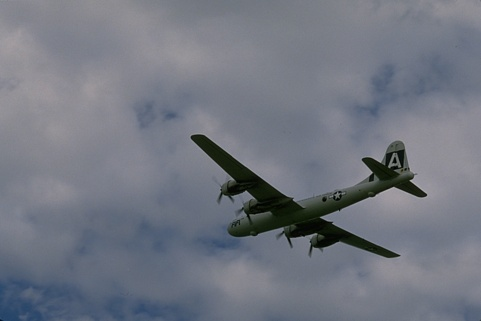
\includegraphics[height=120pt, width=140pt]{segmentaciones/3096.jpg}}
	\hspace{3mm}
	\subfigure[Ground truth]{
\includegraphics[height=120pt, width=140pt]{segmentaciones/3096.png}}
	\hspace{3mm}
	\subfigure[Segmentaci\'on ($k=30000$)]{
\includegraphics[height=120pt, width=140pt]{segmentaciones/3096_seg.jpg}}
	\caption{}
	\end{center}
	\label{Fscores}
\end{figure}
\vspace{-7mm} 
No es sorprendente que una imagen de esta índole, cuyos contornos son fáciles de distinguir y con iluminaci\'on uniforme, sea la que produzca un mejor resultado. De todas formas el algoritmo sigue siendo susceptible a ciertos patrones como el cambio entre cielo y nubes, que le agregan ruido indeseado. Queda como trabajo futuro analizar si con esta implementaci\'on es posible modificar la funci\'on $\tau$ para evitar este comportamiento. Notar que si no se tomase como restricci\'on considerar \'unicamente los píxeles ``borde'' im\'agenes como esta tendr\'ian valores de \textit{Precision}$\approx 1$ debido a la gran componente del fondo. \\
\indent A su vez podemos observar la imagen que para la mayor\'ia de los valores de $k$ obtuvo el peor valor de $F_2$
\begin{figure}[H]
	\begin{center}
	\subfigure[Imagen original]{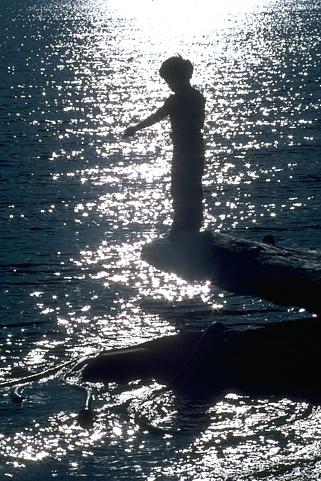
\includegraphics[height=120pt, width=140pt]{segmentaciones/26031.jpg}}
	\hspace{3mm}
	\subfigure[Ground truth]{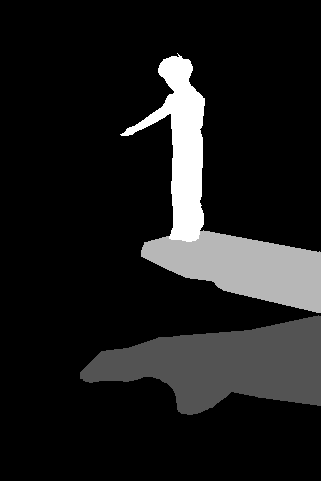
\includegraphics[height=120pt, width=140pt]{segmentaciones/26031.png}}
	\hspace{3mm}
	\subfigure[Segmentaci\'on ($k=30000$)]{
\includegraphics[height=120pt, width=140pt]{segmentaciones/26031_seg.jpg}}
	\caption{}
	\end{center}
	\label{Fscores}
\end{figure}
\vspace{-7mm} 

\indent Esta presenta muchos problemas para nuestro algoritmo por la alta variabilidad de colores que genera la luz. Es argumentable que el objeto de interés de esta imagen es el sujeto erguido, y en segundo plano las rocas y el agua. El algoritmo junt\'o al sujeto y las rocas mientras que el agua la separo basado en la iluminaci\'on que esta recible. Se podr\'ia decir que para este tipo de fotos la segmentaci\'on no es la esperada.
 

\subsection{Distintas aplicaciones y an\'alisis cualitativo}
Si bien el algoritmo es correcto respecto a su especificaci\'on y cumple las propiedades propuestas, el objetivo de la segmentaci\'on es poder diferenciar un objeto de estudio para un conjunto de im\'agenes que cumplen alguna particularidad. A continuaci\'on se tuvieron en cuenta distintos problemas que se pueden resolver utilizando segmentacion de im\'agenes y se evalu\'o si el algoritmo implementado pudiese ser de utilidad para estos casos.

\subsubsection{Reconocimiento de transeúntes}
Una de las nuevas tecnolog\'ias en desarrollo es la de autmóviles autónomos. Uno de los desaf\'ios que presenta es el reconocimiento de sujetos en la calle, a fin de evitar accidentes. En parte este problema se podr\'ia resolver utilizando una segmentaci\'on en tiempo real, junto con un clasificador del objeto segmentado. \\
Tomando im\'agenes de la \textit{Penn-Fudan Database for Pedestrian Detection and Segmentation} \footnote{\url{https://www.cis.upenn.edu/~jshi/ped_html/#pub1}} podemos evaluar el comportamiento del algoritmo sobre instancias reales.
\begin{figure}[H]
	\begin{center}
	\subfigure[]{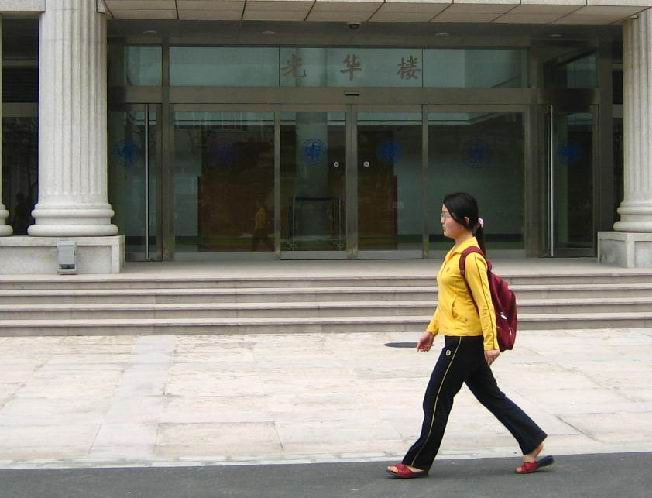
\includegraphics[height=110pt, width=110pt]{segmentaciones/call1.jpg}}
	\subfigure[$k=12000$]{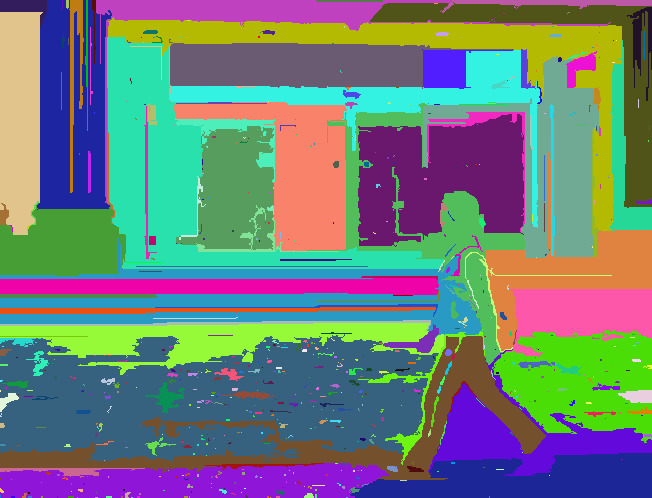
\includegraphics[height=110pt, width=110pt]{segmentaciones/call1_seg.jpg}}
	\hspace{3mm}
	\subfigure[]{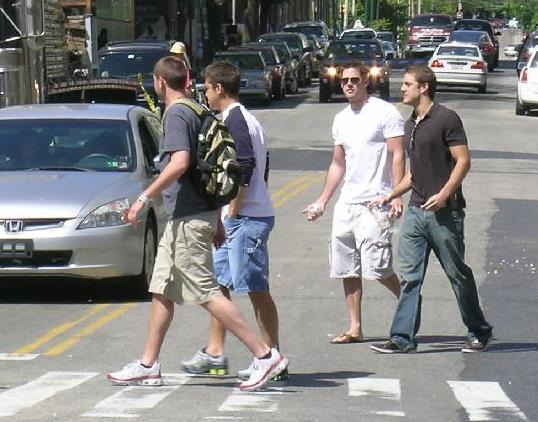
\includegraphics[height=110pt, width=110pt]{segmentaciones/call2.jpg}}
	\subfigure[$k=12000$]{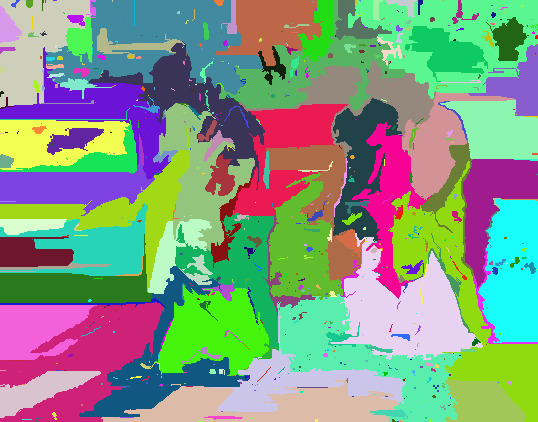
\includegraphics[height=110pt, width=110pt]{segmentaciones/call2_seg.jpg}}
	\caption{}
	\end{center}
	\label{Rec_tran}
\end{figure}
\vspace{-7mm}

\indent Evidentemente el comportamiento no es el requerido, mucha informaci\'on de los fondos afecta negativamente sobre el objeto de estudio y no es distinguible fácilmente. Se podr\'ia considerar tomar un valor de $k$ mayor, pero esto tampoco funcionar\'ia ya que en la subfigura \textit{(b)} ya hay componentes que son la junta de dos partes distintas, como es el caso de la mochila y las escaleras del fondo. Mismo en la subfigura \textit{(d)} la mayor parte de las cosas es irreconocible en la segmentaci\'on.

\subsubsection{Divisi\'on de rasgos faciales}
En varias aplicaciones puede ser de interés reconocer rasgos faciales de un individuo, como por ejemplo en filtros de im\'agenes hasta reconocimiento de gente desaparecida. Tomando algunas fotos de un \textit{dataset} \footnote{\url{http://pics.psych.stir.ac.uk/2D_face_sets.htm}} podemos analizar el comportamiento de las segmentaciones.
\begin{figure}[H]
	\begin{center}
	\subfigure[]{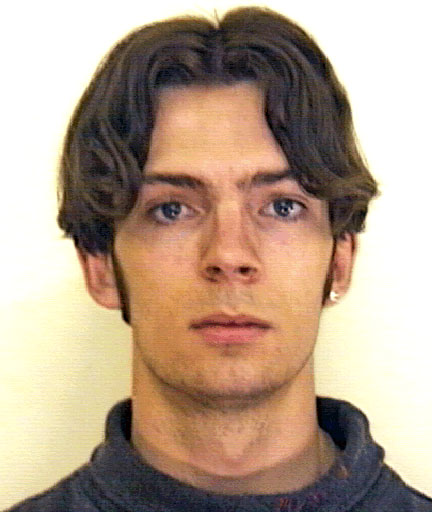
\includegraphics[height=110pt, width=110pt]{segmentaciones/cara1.jpg}}
	\subfigure[$k=10000$]{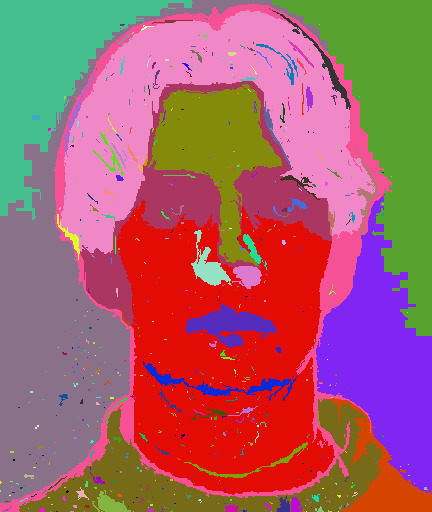
\includegraphics[height=110pt, width=110pt]{segmentaciones/cara1_seg.jpg}}
	\hspace{3mm}
	\subfigure[]{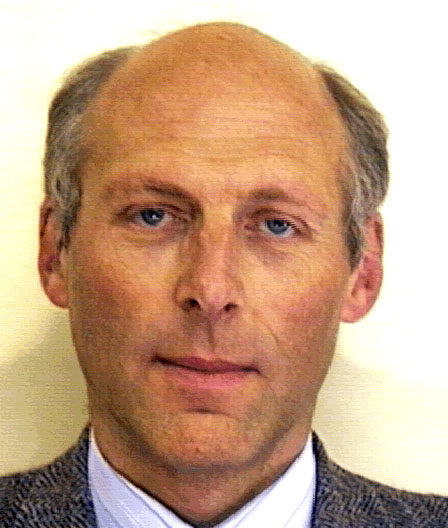
\includegraphics[height=110pt, width=110pt]{segmentaciones/cara2.jpg}}
	\subfigure[$k=10000$]{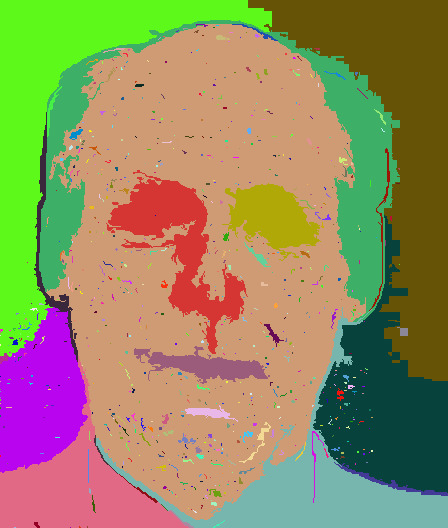
\includegraphics[height=110pt, width=110pt]{segmentaciones/cara2_seg.jpg}}
	\caption{}
	\end{center}
\end{figure}
\vspace{-7mm}

\indent En comparaci\'on' al problema de reconocimiento de transeúntes, el algoritmo parece funcionar mejor para esta tarea. Vemos como ciertos aspectos como el pelo de las personas se encuentra bien delimitado, las bocas se pueden distinguir aunque con algo de ruido y partes como los ojos quedan sumidos en otras componentes. Si bien no parecer\'ia ser aplicable al problema propuesto, el rendimiento parece mejorar para este problema que se podr\'ia decir m\'as simple.  


\subsubsection{Identificaci\'on de núcleos celulares}
Uno de los ambientes en donde m\'as se trabaja con procesamiento de im\'agenes digitales es en el \'area de la medicina.  Reconocimiento de tejidos, tumores y separaci\'on de celulas de im\'agenes microscópicas son algunas de las tareas que se resuelven al d\'ia de hoy, aunque generalmente con un acercamiento desde lo que se conoce como \textit{machine learning}. \\
\indent De un \textit{dataset} compuesto de im\'agenes microscópicas de células \footnote{\url{https://nucleisegmentationbenchmark.weebly.com/dataset.html}}, nos interesa ver si el algoritmo implementado es capaz de separar los l\'imites entre las células y sus n\'ucleos. Esta tarea requiere de una precisi\'on mayor a las anteriores debido a que no hay una sola aparici\'on del objeto de estudio en las im\'agenes, y con esto en mente se tomaron valores de $k$ mucho m\'as chicos que los que se utilizaron para el resto de las experimentaciones.
\begin{figure}[H]
	\begin{center}
	\subfigure[]{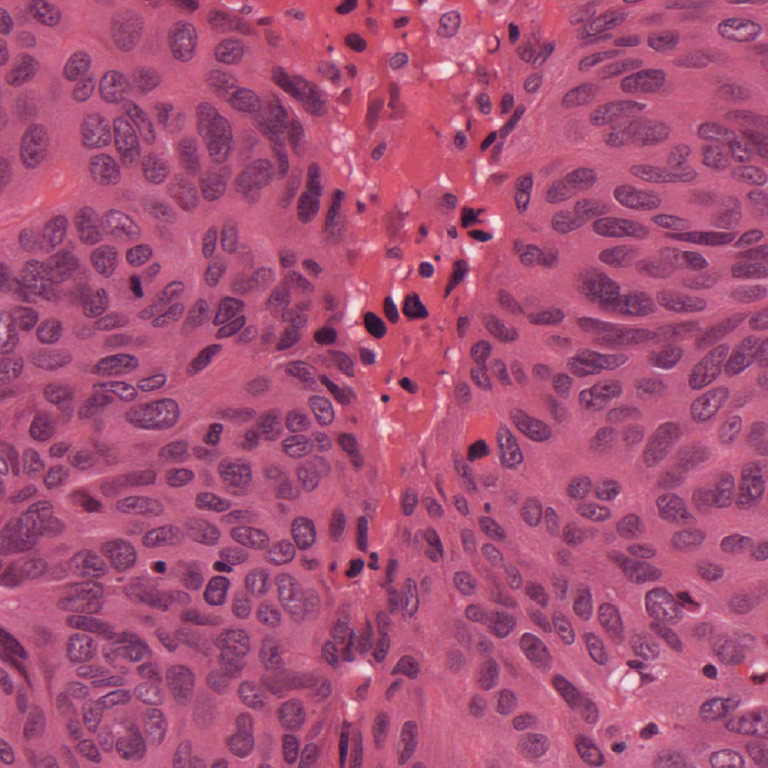
\includegraphics[height=110pt, width=110pt]{segmentaciones/cell1.jpg}}
	\subfigure[$k=80$]{
\includegraphics[height=110pt, width=110pt]{segmentaciones/cell1_seg.jpg}}
	\hspace{3mm}
	\subfigure[]{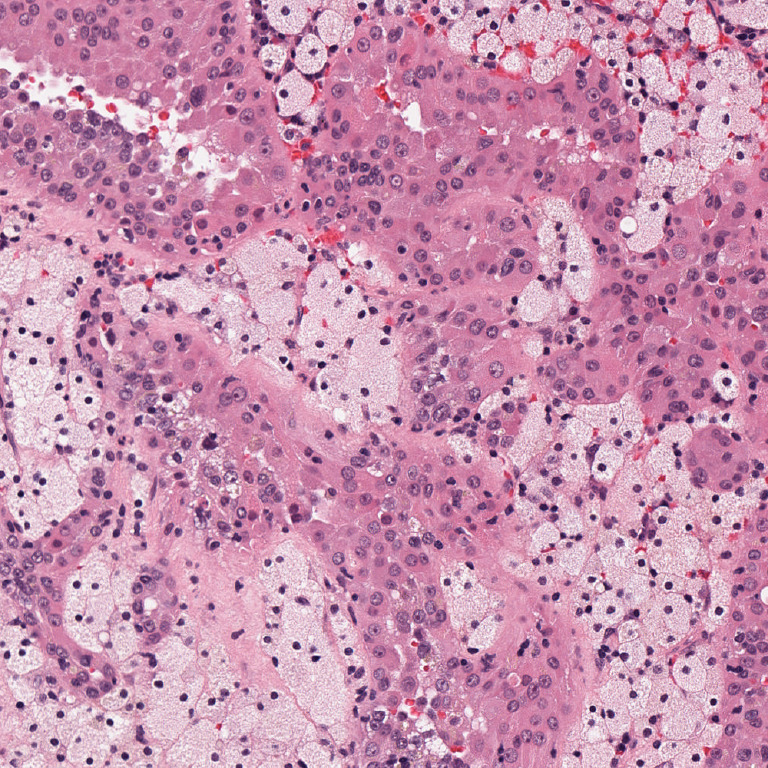
\includegraphics[height=110pt, width=110pt]{segmentaciones/cell2.jpg}}
	\subfigure[$k=1000$]{
\includegraphics[height=110pt, width=110pt]{segmentaciones/cell2_seg.jpg}}
	\caption{}
	\end{center}
\end{figure}
\vspace{-7mm}

\indent Luego de ver las segmentaciones generadas, no hay duda que esta no es una aplicaci\'on viable para el algoritmo. Ambos resultados son incomparables con las im\'agenes originales, haciendo imposible cualquier reconocimiento de secciones relevantes. En definitiva: el algoritmo no es apto para resolver problemas que requieran un alto grado de detalle. 
\clearpage

\section{Conclusión y trabajos futuros}

A lo largo del trabajo se observ\'o que el m\'etodo propuesto es considerablemente eficiente en lo que respecta al tiempo de c\'omputo, pero no se pudo encontrar una aplicaci\'on especifica en la que su desempe\~no como separador de objetos resulte útil. De todas formas se pudo comprobar experimentalmente que lo propuesto en \cite{Felzenszwalb2004} se cumpl\'ia y que la m\'etrica propuesta en este trabajo reflejaba suficientemente bien lo planteado en \cite{li2013benchmark}. \\
\indent Algunas de las cosas sobre las que se podr\'ia trabajar a futuro son considerar una nueva funci\'on de \textit{threshold} que proporcione mejores resultados en cuanto a la segmentaci\'on y evaluar si el tiempo de c\'omputo resultante sigue siendo bueno o por lo menos aceptable. También resta encontrar alguna aplicaci\'on en donde la segmentaci\'on sea lo suficientemente buena para resolver un problema m\'as complejo. 
\clearpage


\end{document}
